\documentclass{article}

\usepackage{amsmath}
\usepackage{amsfonts}
\usepackage{amssymb}
\usepackage{booktabs}
\usepackage{geometry}
\usepackage{graphicx}
\usepackage{tcolorbox}
\usepackage{tikz}
\usepackage{xcolor}

\usetikzlibrary{arrows.meta, calc, patterns, positioning}

\geometry{a4paper, margin=1in}

\newcommand{\notesetup}[1]{
    \title{#1}
    \author{}
    \date{}
}

\newtcolorbox{keyidea}[1]{
    colback=blue!5,
    colframe=blue!45!black,
    title=#1
}

\newtcolorbox{pitfall}[1]{
    colback=red!4,
    colframe=red!55!black,
    title=#1
}


\begin{document}

\notesetup{Mechanical Energy, Conservation, and Efficiency}
\maketitle

\section{Why Mechanical Energy Matters}
In the previous lesson, work was introduced as a way to transfer energy. In this lesson, we make that idea more precise:
\begin{itemize}
    \item work is a \textbf{process}
    \item energy is a \textbf{property of a system}
    \item when work is done on a system, the system's energy changes
\end{itemize}

For Grade 11 mechanics, the two most important forms are:
\begin{itemize}
    \item \textbf{gravitational potential energy}: energy due to height
    \item \textbf{kinetic energy}: energy due to motion
\end{itemize}

These two forms combine to give \textbf{mechanical energy}.

\begin{keyidea}{Main Goal}
Mechanical energy lets us analyze motion by comparing the energy at the start and at the end of a process, instead of tracking every force at every moment.
\end{keyidea}

\section{From Work to Energy Changes}
The central bridge in this chapter is:

\begin{keyidea}{Bridge Idea}
Work transfers energy. When work is done on a system, the system's energy changes.
\end{keyidea}

This idea leads naturally to two important results:
\begin{itemize}
    \item net work changes \textbf{kinetic energy}
    \item work done against gravity changes \textbf{gravitational potential energy}
\end{itemize}

\subsection{Net Work and Kinetic Energy}
Start with the expression for work by a constant force parallel to the motion:
\begin{equation*}
    W = F \Delta d
\end{equation*}

Use Newton's second law, $F = ma$:
\begin{equation*}
    W_{\text{net}} = ma \Delta d
\end{equation*}

From kinematics,
\begin{equation*}
    v_f^2 = v_i^2 + 2a \Delta d
    \quad \Rightarrow \quad
    a \Delta d = \frac{v_f^2 - v_i^2}{2}
\end{equation*}

Substitute into the work equation:
\begin{equation*}
    W_{\text{net}} = m\left( \frac{v_f^2 - v_i^2}{2} \right)
\end{equation*}
\begin{equation*}
    W_{\text{net}} = \frac{1}{2}mv_f^2 - \frac{1}{2}mv_i^2
\end{equation*}

This shows that net work changes the quantity $\frac{1}{2}mv^2$. We define that quantity as \textbf{kinetic energy}:
\begin{equation}
    E_k = \frac{1}{2}mv^2
\end{equation}

So the work-energy relationship is:
\begin{equation}
    W_{\text{net}} = \Delta E_k
\end{equation}

\subsection{Work Done Against Gravity and Potential Energy}
If an object is lifted upward at constant speed, the applied force equals the object's weight:
\begin{equation*}
    F = mg
\end{equation*}

The work done by the lifting force through a height $\Delta h$ is:
\begin{equation*}
    W = F \Delta h = mg \Delta h
\end{equation*}

This work increases the stored energy of the object-Earth system. So we define the change in gravitational potential energy as:
\begin{equation}
    \Delta E_g = mg \Delta h
\end{equation}

If we choose a reference level where $E_g = 0$, then this becomes:
\begin{equation}
    E_g = mgh
\end{equation}

\section{Gravitational Potential Energy ($E_g$)}
An object raised above a reference level has stored energy because gravity can cause it to move downward.

The formula
\begin{equation*}
    E_g = mgh
\end{equation*}
comes from the work required to raise the object against gravity.

Where:
\begin{itemize}
    \item $E_g$ is gravitational potential energy, measured in joules ($\text{J}$)
    \item $m$ is mass, measured in kilograms ($\text{kg}$)
    \item $g = 9.8\,\text{N/kg}$
    \item $h$ is the height above the chosen reference level, measured in metres ($\text{m}$)
\end{itemize}

\subsection{Reference Level}
The value of $h$ depends on where we choose the zero level.

\begin{itemize}
    \item The \textbf{reference level} is the height where we define $E_g = 0$.
    \item Different choices of zero are allowed.
    \item The important quantity is usually the \textbf{change} in gravitational potential energy.
\end{itemize}

\begin{pitfall}{Common Mistake}
Students often think there is only one correct zero level for gravitational potential energy. There is not. You may choose any convenient reference level, as long as you use it consistently.
\end{pitfall}

\begin{figure}[h]
    \centering
    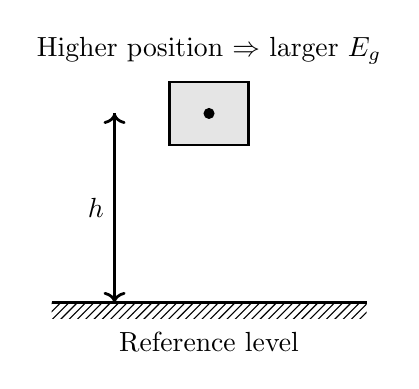
\begin{tikzpicture}[scale=1.0, line width=1pt]
        \draw[thick] (-2,0) -- (2,0);
        \fill[pattern=north east lines] (-2,-0.2) rectangle (2,0);
        \draw[fill=gray!20] (-0.5,2.0) rectangle (0.5,2.8);
        \fill (0,2.4) circle (2pt);
        \draw[dashed] (-1.2,2.4) -- (-1.2,0);
        \draw[<->] (-1.2,0) -- (-1.2,2.4) node[midway,left] {$h$};
        \node at (0,-0.5) {Reference level};
        \node at (0,3.2) {Higher position $\Rightarrow$ larger $E_g$};
    \end{tikzpicture}
    \caption{Gravitational potential energy depends on the chosen reference level.}
\end{figure}

\subsection*{Sample Problem 1: Gravitational Potential Energy}
\textbf{Problem:} A $4.0\,\text{kg}$ toolbox is placed on a shelf $1.8\,\text{m}$ above the floor. What is its gravitational potential energy relative to the floor?

\textbf{Solution:}
\begin{equation*}
    E_g = mgh
\end{equation*}
\begin{equation*}
    E_g = (4.0)(9.8)(1.8) \approx 71\,\text{J}
\end{equation*}

\section{Kinetic Energy ($E_k$)}
Any moving object has kinetic energy.

The formula
\begin{equation*}
    E_k = \frac{1}{2}mv^2
\end{equation*}
comes from combining the definitions of work, force, and acceleration.

Where:
\begin{itemize}
    \item $E_k$ is kinetic energy, measured in joules ($\text{J}$)
    \item $m$ is mass, measured in kilograms ($\text{kg}$)
    \item $v$ is speed, measured in meters per second ($\text{m/s}$)
\end{itemize}

Since speed is squared, kinetic energy is always zero or positive.

\begin{keyidea}{Speed Matters a Lot}
If speed doubles, kinetic energy becomes four times as large.
\end{keyidea}

\subsection*{Sample Problem 2: Kinetic Energy}
\textbf{Problem:} A $0.80\,\text{kg}$ ball moves at $6.0\,\text{m/s}$. What is its kinetic energy?

\textbf{Solution:}
\begin{equation*}
    E_k = \frac{1}{2}mv^2
\end{equation*}
\begin{equation*}
    E_k = \frac{1}{2}(0.80)(6.0)^2 = 14.4\,\text{J}
\end{equation*}

\section{Mechanical Energy}
The total of gravitational potential energy and kinetic energy is called \textbf{mechanical energy}.

\begin{equation}
    E_{\text{mech}} = E_g + E_k
\end{equation}

In many Grade 11 problems, this is the most useful total to track.

\subsection{Why Add These Two Together?}
These are the two main forms of energy that keep exchanging in simple mechanics problems:
\begin{itemize}
    \item height gives gravitational potential energy
    \item motion gives kinetic energy
\end{itemize}

If energy is only moving back and forth between these two forms, then their sum is the quantity that stays constant.

\subsection{Mechanical Energy in Motion}
\begin{itemize}
    \item At a high point, an object may have large $E_g$ and small $E_k$.
    \item As it falls, $E_g$ decreases and $E_k$ increases.
    \item If friction is negligible, the total mechanical energy stays the same.
\end{itemize}

\begin{figure}[h]
    \centering
    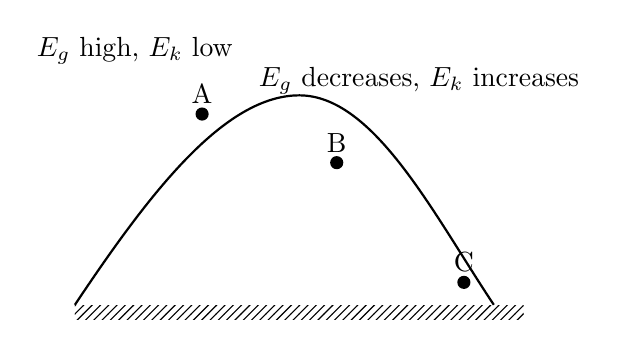
\begin{tikzpicture}[scale=0.95, line width=1pt]
        \draw[thick] (-2,0) .. controls (-1,1.5) and (0,2.8) .. (1.0,2.8)
                     .. controls (2.0,2.8) and (2.8,1.2) .. (3.6,0);
        \fill[pattern=north east lines] (-2,-0.2) rectangle (4,-0.01);

        \fill (-0.3,2.55) circle (2.5pt);
        \node[above] at (-0.3,2.55) {A};

        \fill (1.5,1.9) circle (2.5pt);
        \node[above] at (1.5,1.9) {B};

        \fill (3.2,0.3) circle (2.5pt);
        \node[above] at (3.2,0.3) {C};

        \node at (-1.2,3.4) {$E_g$ high, $E_k$ low};
        \node at (2.6,3.0) {$E_g$ decreases, $E_k$ increases};
    \end{tikzpicture}
    \caption{As an object moves downhill, gravitational potential energy changes into kinetic energy.}
\end{figure}

\subsection*{Sample Problem 3: Total Mechanical Energy}
\textbf{Problem:} A $2.0\,\text{kg}$ object is moving at $5.0\,\text{m/s}$ at a height of $3.0\,\text{m}$ above the ground. Find its total mechanical energy relative to the ground.

\textbf{Solution:}
\begin{equation*}
    E_g = mgh = (2.0)(9.8)(3.0) = 58.8\,\text{J}
\end{equation*}
\begin{equation*}
    E_k = \frac{1}{2}mv^2 = \frac{1}{2}(2.0)(5.0)^2 = 25\,\text{J}
\end{equation*}
\begin{equation*}
    E_{\text{mech}} = E_g + E_k = 58.8 + 25 = 83.8\,\text{J}
\end{equation*}

\section{Conservation of Mechanical Energy}
If friction and air resistance are negligible, then mechanical energy is conserved.

\begin{equation}
    E_{g,i} + E_{k,i} = E_{g,f} + E_{k,f}
\end{equation}

This is a direct consequence of the work-energy ideas above. If no significant energy is transferred away as thermal energy or sound, then energy only changes between $E_g$ and $E_k$.

\begin{keyidea}{When Can You Use Conservation?}
Use conservation of mechanical energy when energy is changing mainly between gravitational potential energy and kinetic energy, and non-conservative effects such as friction are negligible.
\end{keyidea}

\subsection{Typical Situations}
\begin{itemize}
    \item an object falling freely
    \item a roller coaster moving on a nearly frictionless track
    \item a pendulum moving through a short interval with little air resistance
\end{itemize}

\subsection*{Sample Problem 4: Falling Object}
\textbf{Problem:} A ball is dropped from rest from a height of $2.5\,\text{m}$. Ignore air resistance. What is its speed just before hitting the ground?

\textbf{Solution:}
Choose the ground as the reference level. Then
\begin{equation*}
    E_{g,i} + E_{k,i} = E_{g,f} + E_{k,f}
\end{equation*}
\begin{equation*}
    mgh + 0 = 0 + \frac{1}{2}mv^2
\end{equation*}
Mass cancels:
\begin{equation*}
    gh = \frac{1}{2}v^2
\end{equation*}
\begin{equation*}
    v = \sqrt{2gh} = \sqrt{2(9.8)(2.5)} = 7.0\,\text{m/s}
\end{equation*}

\subsection{When Mechanical Energy Is Not Conserved}
If friction or air resistance is important, then some mechanical energy changes into other forms such as thermal energy or sound.

\begin{pitfall}{Important Distinction}
If mechanical energy decreases, that does \textbf{not} mean total energy is destroyed. It means some of the mechanical energy has been transformed into other forms.
\end{pitfall}

\subsection*{Sample Problem 5: Loss of Mechanical Energy}
\textbf{Problem:} A ball is dropped from $1.5\,\text{m}$ and bounces back to a height of $1.2\,\text{m}$. Has energy been lost?

\textbf{Solution:}
The ball's \textbf{mechanical} energy after the bounce is smaller because it does not return to the original height. Some of the original mechanical energy has been transformed into thermal energy and sound during the collision. Total energy is still conserved.

\section{Efficiency}
Real devices do not usually transfer all input energy into useful output energy.

Efficiency belongs naturally at the end of this chapter because it measures how much of the input work or energy ends up in the form we actually want.

\begin{equation}
    \text{efficiency} = \frac{E_{\text{out}}}{E_{\text{in}}} \times 100\%
\end{equation}

Where:
\begin{itemize}
    \item $E_{\text{in}}$ is the input energy
    \item $E_{\text{out}}$ is the useful output energy
\end{itemize}

\subsection{What Efficiency Tells You}
\begin{itemize}
    \item High efficiency means most of the input energy becomes useful output.
    \item Low efficiency means a large fraction becomes less useful forms such as thermal energy.
\end{itemize}

\subsection*{Sample Problem 6: Efficiency of a Ramp}
\textbf{Problem:} A worker uses a ramp to push a $60\,\text{kg}$ crate onto a platform $0.80\,\text{m}$ high. The worker does $650\,\text{J}$ of input work. What is the efficiency of the ramp system?

\textbf{Solution:}
The useful output energy is the gain in gravitational potential energy:
\begin{equation*}
    E_{\text{out}} = mgh = (60)(9.8)(0.80) = 470.4\,\text{J}
\end{equation*}
Then
\begin{equation*}
    \text{efficiency} = \frac{470.4}{650}\times 100\% \approx 72\%
\end{equation*}

\section{Quick Concept Check}
\begin{enumerate}
    \item If a skier moves downhill, what happens to $E_g$ and $E_k$?
    \item Can two students choose different reference levels and still solve the same problem correctly?
    \item When can you use conservation of mechanical energy?
    \item If a machine is $100\%$ efficient, what does that mean physically?
\end{enumerate}

\section{Summary}
\begin{itemize}
    \item Gravitational potential energy: $E_g = mgh$
    \item Kinetic energy: $E_k = \frac{1}{2}mv^2$
    \item Mechanical energy: $E_{\text{mech}} = E_g + E_k$
    \item If friction is negligible, mechanical energy is conserved:
    \begin{equation*}
        E_{g,i} + E_{k,i} = E_{g,f} + E_{k,f}
    \end{equation*}
    \item If mechanical energy decreases, some energy has usually been transformed into thermal energy or sound.
    \item Efficiency is the ratio of useful output energy to input energy.
\end{itemize}

\end{document}
